% !TEX root = main.tex

\section{Experiments}

This section will explore the same example given by the original paper, which is called ``friends and smokers'' problem. We will firstly how the definition of this example respect to the symbols we use before. Then two experiments will be deducted on knowledge base with only observed facts and knowledge base with extra rules. Finally, we will show the effects of vector length.

\subsection{Friends and Smokers}
\begin{itemize}
    \item Constant $C=C1 \cup C2=\{a,b,c,d,e,f,g,h\}\cup \{a,b,c,d,e,f,g,h\}$ is all people in two groups $C1$ and $C2$
    \item Functions: $S/1$, whether a person smokes; $F/2$, whether two persons are friends; $C/1$, whether a person have cancer.
    \item Predicate: all components of all clauses, including $F/2$, $S/1$ and $C/1$
    \item Clause: original clauses is defined as the yellow part of Figure.\ref{fig:example}. We need transfer them into disjunctive form.
\end{itemize}

The value of ``observed facts'' we know is shown in Figure.\ref{fig:example}.

\begin{figure*}
    \centering
    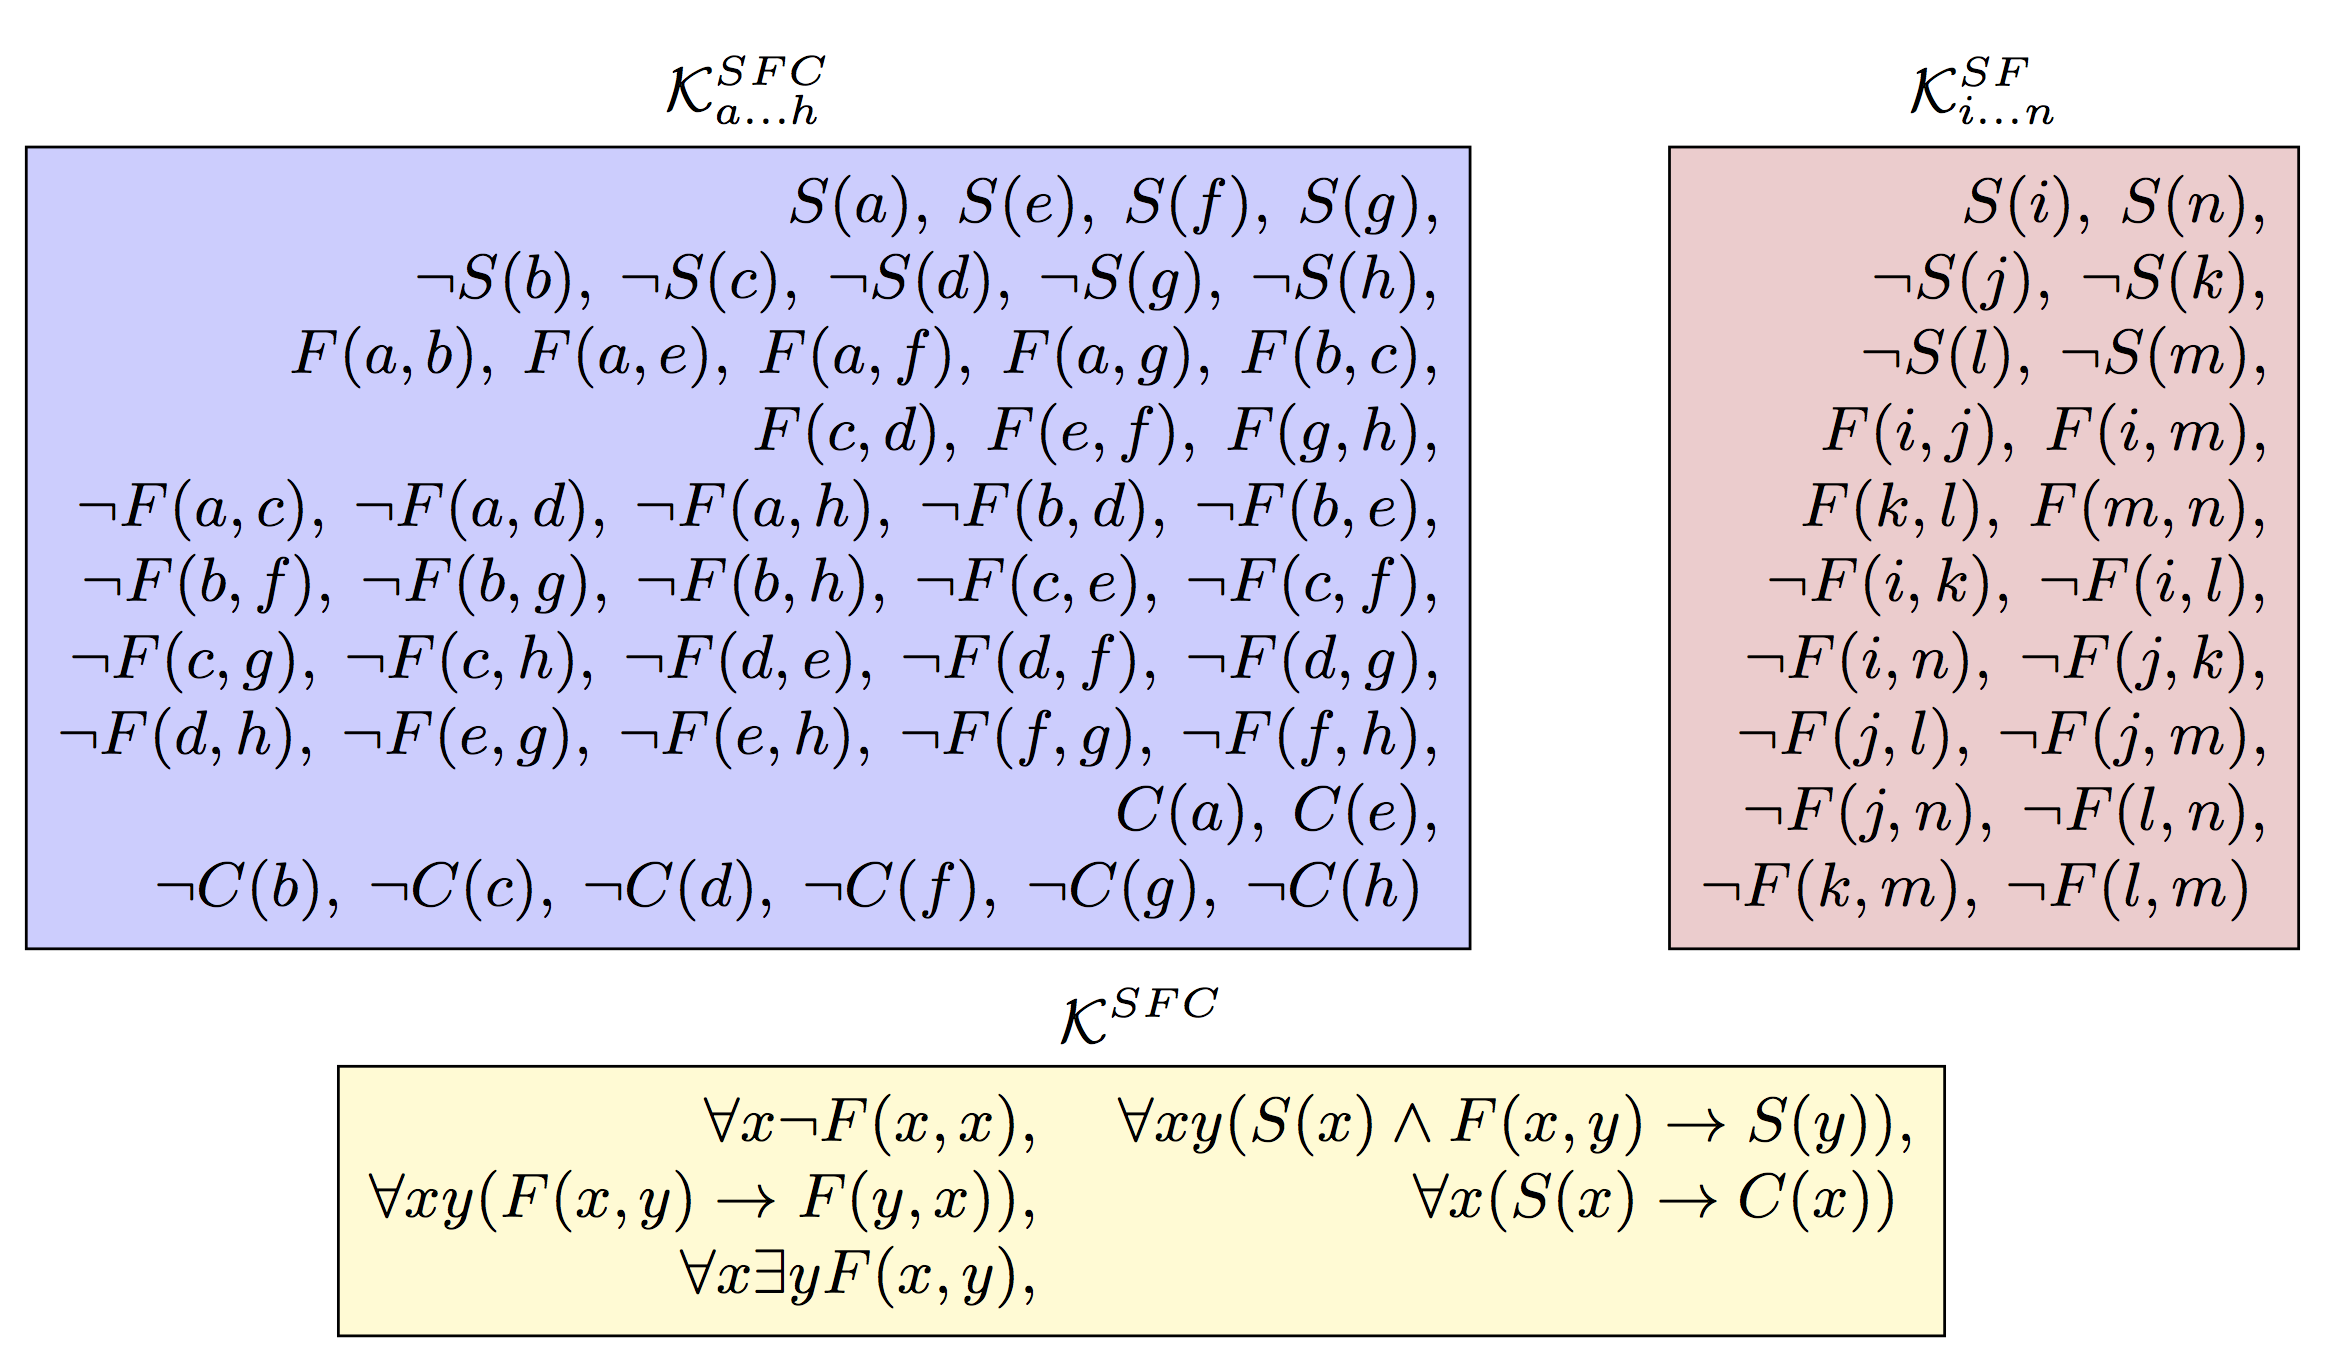
\includegraphics[width=.7\textwidth]{img/example.png}
    \caption{Friends and Smokers}
    \label{fig:example}
\end{figure*}

\subsection{Fit Knowledge Base}

\begin{figure*}[!]
    \centering
    % \vspace{-0.2em}
    \begin{subfigure}[]{0.33\textwidth}
        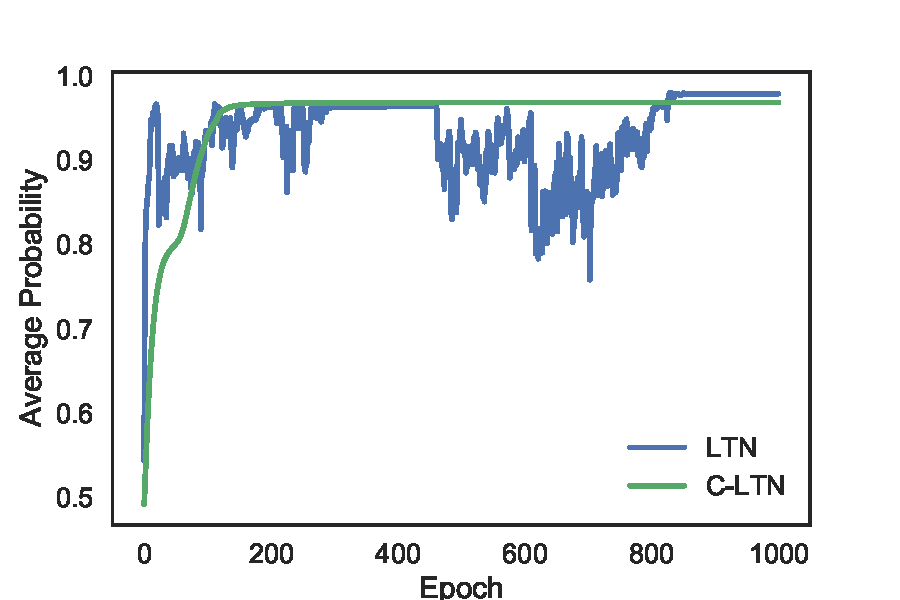
\includegraphics[width=\textwidth]{img/curve1.pdf}
        \caption{Probability w.r.t. Epoch}
        \label{fig:fitting-prob-epoch}
        %\vspace{-0.3em}
    \end{subfigure}~~~~
    \begin{subfigure}[]{0.33\textwidth}
        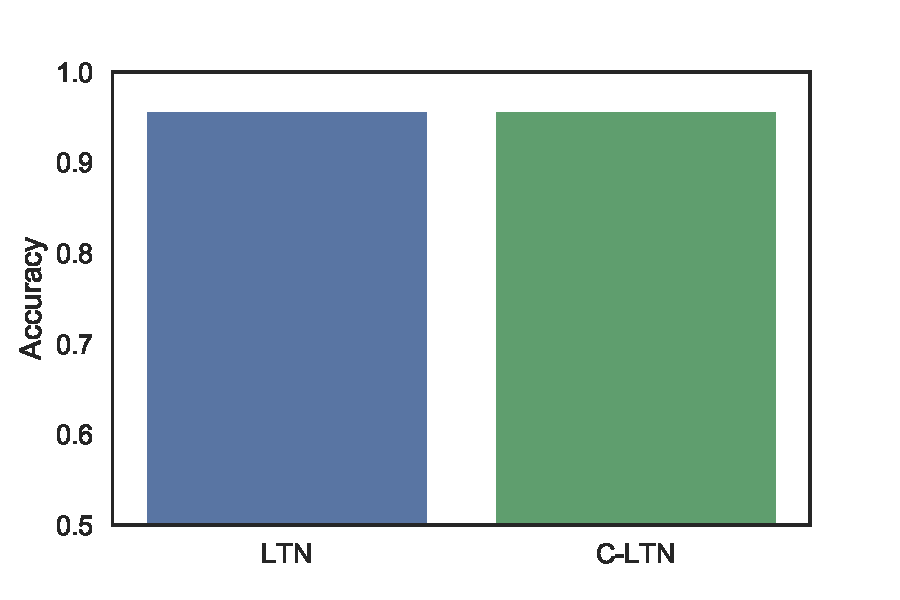
\includegraphics[width=\textwidth]{img/bar1.pdf}
        \caption{Best Accuracy on Group1}
        \label{fig:fitting-best-accuracy-1}
        %\vspace{-0.3em}
    \end{subfigure}~~~~
    \begin{subfigure}[]{0.33\textwidth}
        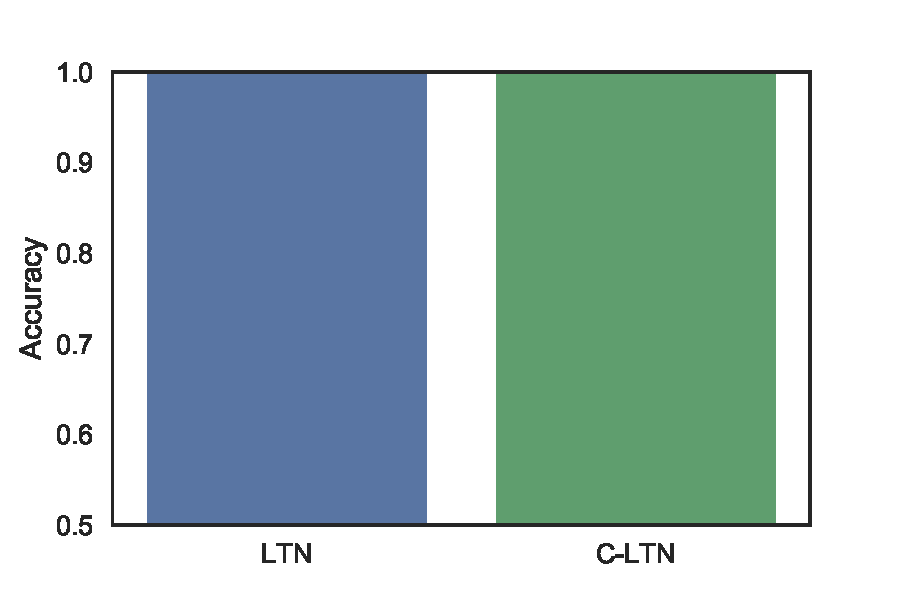
\includegraphics[width=\textwidth]{img/bar2.pdf}
        \caption{Best Accuracy on Group2}
        \label{fig:fitting-best-accuracy-2}
        %\vspace{-0.8em}
    \end{subfigure}
    \caption{Fitting Observed Facts.}
    \label{fig:fitting}
    % \vspace{-1.2em}
\end{figure*}

In this experiment, we only use the oberserved facts, which is $K_{exp1} = K^{SFC}_{a \dots h} \cup K^{SF}_{i\dots n}$.

As there is no rules in this part, so we only compare the result of LTN and C-LTN.
Figure \ref{fig:fitting} shows the result of this experiment, where Figure \ref{fig:fitting-prob-epoch} is the probability change with respect to the training epoch, Figure \ref{fig:fitting-best-accuracy-1} shows the accuracy on the first group and Figure \ref{fig:fitting-best-accuracy-2} is that of the second group.

From the Figure \ref{fig:fitting}, it's clear that both LTN and C-LTN fit the observed data very well. The reason why the accuracy on first group is not $100\%$ is that there exists a contradictory pair: $S(g)$ and $\neg S(g)$. So it's not possible to make both of them $100\%$ true.

% Another interesting phenomenon is thay

\subsection{Learn From Rule}

\begin{figure*}[!]
    \centering
    % \vspace{-0.2em}
    \begin{subfigure}[]{0.33\textwidth}
        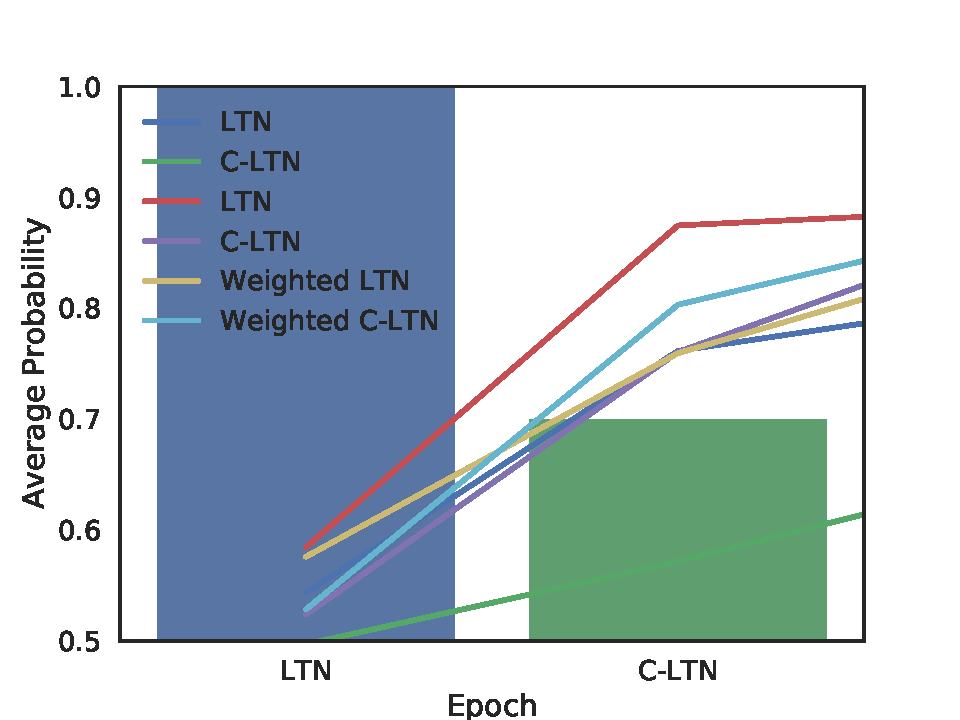
\includegraphics[width=\textwidth]{img/curve2.pdf}
        \caption{Probability w.r.t. Epoch}
        \label{fig:learning-prob-epoch}
        %\vspace{-0.3em}
    \end{subfigure}~~~~
    \begin{subfigure}[]{0.33\textwidth}
        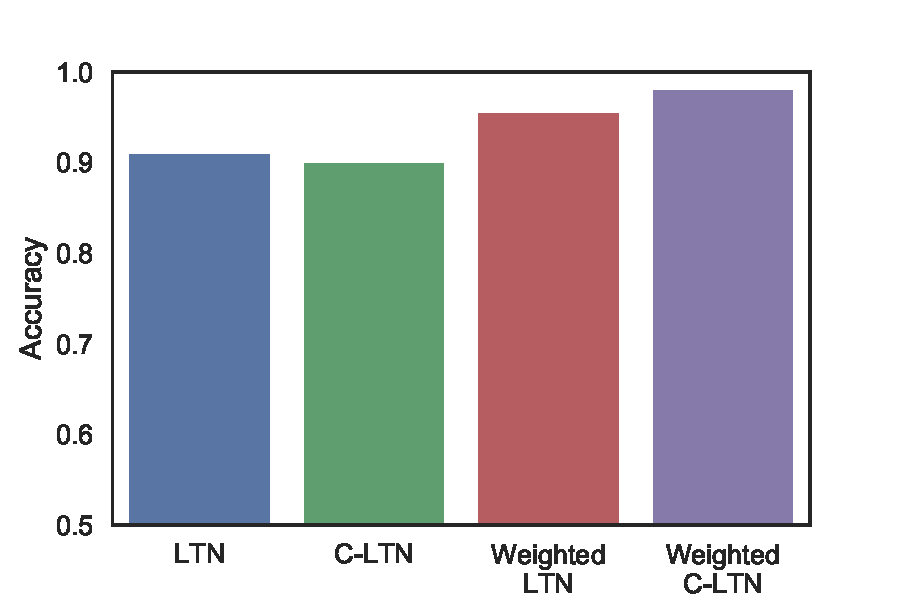
\includegraphics[width=\textwidth]{img/bar3.pdf}
        \caption{Best Accuracy on Group1}
        \label{fig:learning-best-accuracy-1}
        %\vspace{-0.3em}
    \end{subfigure}~~~~
    \begin{subfigure}[]{0.33\textwidth}
        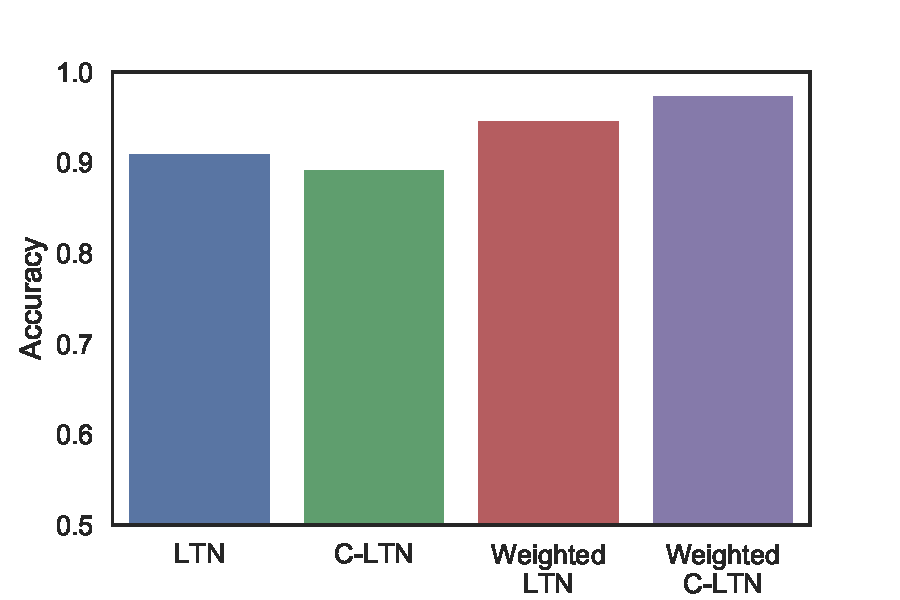
\includegraphics[width=\textwidth]{img/bar4.pdf}
        \caption{Best Accuracy on Group2}
        \label{fig:learning-best-accuracy-2}
        %\vspace{-0.8em}
    \end{subfigure}
    \caption{Learning from Observed Facts \& Rules.}
    \label{fig:learning}
    % \vspace{-1.2em}
\end{figure*}

Firgure \ref{fig:learning} shows the result of two models on datasets. Like the result in last subsection, this figure containts three subfigures, including probability changes and best accuracy on two groups.

Some interesting phenomenon can be concluded from the results.

First, by comparing results on weighted and unweighted dataset, we can see that training on weighted dataset gets a better performance.
As we said before, this is because the weighted method treat each proposal as one clause, which could avoid the unbalanced training.

Second, C-LTN on weighted datasets shows the best performance. That's because CNN has better fitting ability and more stable in training.

\subsection{Parameter Sensitive}

\begin{figure}[!]
    \centering
    % \vspace{-0.2em}
    \begin{subfigure}[]{0.5\textwidth}
        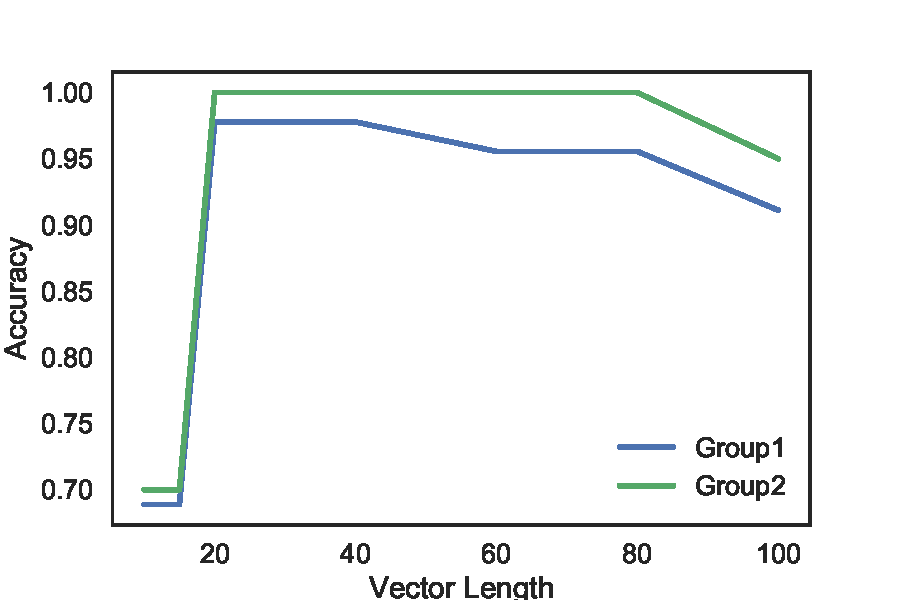
\includegraphics[width=\textwidth]{img/curve3.pdf}
        \caption{Fitting Observed Facts}
        \label{fig:sensitive-best-accuracy-1}
        %\vspace{-0.3em}
    \end{subfigure}

    \begin{subfigure}[]{0.5\textwidth}
        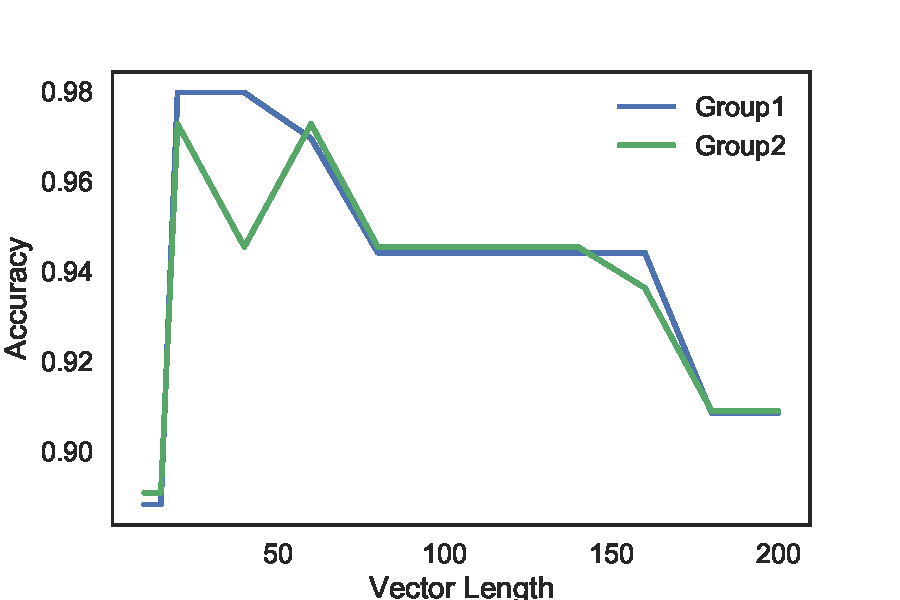
\includegraphics[width=\textwidth]{img/curve4.pdf}
        \caption{Learning from Rules }
        \label{fig:sensitive-best-accuracy-2}
        %\vspace{-0.3em}
    \end{subfigure}
    \caption{Best Accuracy w.r.t. Vector Length.}
    \label{fig:sensitive}
    % \vspace{-1.2em}
\end{figure}

In this part, we want to test the effect of vector length. We enumerate the vector length from 1 to 100 and shows the best accuracy on two groups. We did our experiments on both observed data and weighted dataset with rule. As the performance of C-LNT is better than LNT, we only shows the result of C-LNT, which is shown in Figure \ref{fig:sensitive}.

Figure \ref{fig:fitting-best-accuracy-1} shows the result in observed dataset.
From this figure, we can conclude that the performance is not always getting better with the increase of vector length. That's may because the under training problem. That is, as the 

Actually, we want to find the appropriate vector lenght that is enough for fitting the data
